\section{Drift velocity, drift gap and gas}\label{sec:gas}
\sectionstate{partial}{\texttt{rerun/paper1\_gas/README.md} and \texttt{results/summary.json}, \texttt{twov.json} (bench);
\texttt{rerun/paper1\_spsfigs}, \texttt{sps\_beam\_test\_26/analysis/cloud\_basics} \S16--27 (beam). v2 2026-11-10: the old
section 6 written out as prose and moved in front of the tracking results, which depend on it; the gap paragraph is new;
the SPS gas history moved to \cref{app:beam}.}
\intent{The chamber calibrates itself. The drift velocity is measured two independent ways and the gap a third; they
agree; one physics model with one free number, the water content, describes all of it; and the same analysis sees
oxygen where there is some.}

A TPC turns time into depth through the drift velocity $\vd$, and the angle of a track is
$\tan\theta=w/\vd$, where $w$ is the rate at which the charge of the track moves across the strips as it arrives
(\cref{sec:reco}). Every tracking result of \cref{sec:tracking} therefore rests on $\vd$. No record of the gas on the
bench exists beyond its nominal mixture, Ar/iC$_4$H$_{10}$ 95/5, so the drift velocity has to come from the data. It
does, in two ways that share nothing, and the comparison of the two measures the drift gap.

\subsection{Two velocities and the gap}\label{sec:gap}
The first way uses time alone. A track near normal incidence deposits charge uniformly across the gap, and its signal
summed over all strips lasts from the arrival of the electrons made next to the mesh to that of the electrons made at
the cathode: a drift column of duration $T=g/\vd$, with $g$ the gap (\crefp{fig:twov}{a}). The \emph{timing velocity}
is $g/T$ and needs the gap.

The second way uses the reference tracks and no gap. For inclined tracks the fitted rate $w$ is proportional to the
slope of the reference track, and the constant of proportionality is the drift velocity (\crefp{fig:twov}{b}). We call
it the \emph{angle-scale velocity}, since it is the velocity that makes the fitted angles agree with the reference.

The gap can be had a third way, from geometry: an inclined track crosses the gap over a length $L$ of strips with
$g=L/\tan\theta$, which involves no velocity and gives $28.19\pm0.19$\,mm for chamber~A. The product of the
angle-scale velocity and the column duration is an independent measurement of the same gap. Over the four fields of
chamber~A's drift scan it gives $28.2\pm0.5$\,mm ($\chi^2=4.1$ for 3 degrees of freedom; \crefp{fig:twov}{c}). The
two velocities and the gap therefore close to 2\,\%.

The gap is 1.8\,mm shorter than the 30\,mm of the design, where the aluminium frame is the spacer. The data establish
the mean gap and not its cause. The bow of the readout board (\cref{sec:bow}) cannot be it: a mesh dished away from the
cathode makes the gap longer at the centre, not shorter. The position of the cathode is not measured.
\askStephan{Is a gap of 28.2\,mm at the centre plausible (cathode bulging towards the mesh under the overpressure of the
5\,mm gas gap behind it, frame height)? The other chambers' geometric gaps in our tables are 28.0 (C), 29.4 (D) and
31.1\,mm (B).}
\askDylan{The variation of the gap across chamber~A is not re-derived on the final reconstruction (the July map,
25.7--29.2\,mm, is on a superseded basis), so nothing is said about it. Chamber~E: 30.48\,mm in the configuration,
28.6\,mm geometric, 27.9\,mm used for the SPS gas fit (\cref{app:beam}).}

\begin{figure}[tbp]
  \centering
  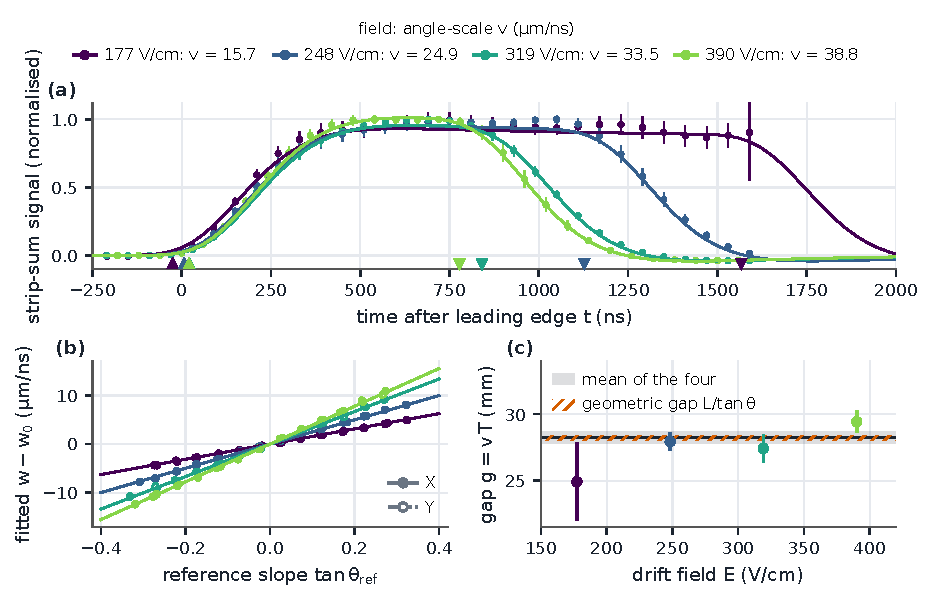
\includegraphics[width=0.9\linewidth]{two_velocities}
  \caption{Two drift velocities and the gap, chamber~A, drift-field scan of 27 June (colour: drift field). (a) Signal
  summed over all strips for tracks near normal incidence, averaged over tracks (points), with the model of a uniform
  column (lines); triangles mark the fitted start and end of the column, whose difference is the drift time
  $T=g/\vd$. (b) Fitted transverse rate $w$, less its offset $w_0$ (\cref{sec:bow}), against the slope of the reference
  track, X filled and Y open; the slope of each line is the angle-scale velocity, which involves no gap. (c) The
  product $g=\vd\,T$ per field: mean $28.2\pm0.5$\,mm (grey band), against the geometric gap $28.19\pm0.19$\,mm
  (hatched), obtained without any drift velocity from the extent in strips of inclined tracks.}
  \label{fig:twov}
\end{figure}

\subsection{Drift velocity against field: one curve, one number}\label{sec:vE}
\Cref{fig:vE} shows both velocities of chamber~A against the drift field. The timing velocity runs from 17.7 to
37.2\,\textmu m/ns between 177 and 390\,V/cm, and the angle-scale velocity from 2.55 to 38.9\,\textmu m/ns over seven
fields. Dry Ar/iC$_4$H$_{10}$ does not describe them: at the fields used here it would drift at about 40\,\textmu m/ns.
A Magboltz~\cite{Biagi1999} calculation with one free number, the water content, does. Fitted to the timing velocity
it gives 0.97\,\% of water (68\,\% interval 0.95--0.99\,\%; $\chi^2=2.5$ for 3 degrees of freedom), and the angle-scale
points, which did not enter the fit, lie within $-1.7$ to $+1.5\,\%$ of that curve.

The other chambers have no field scan, only the drift velocity of their long runs at one field. A single point is
always matched by some water content, so it is not a test of the model; it only expresses the velocity as an
equivalent water, 0.69\,\% for B, 1.00\,\% for C, 0.48\,\% for D and 0.42\,\% for E. It differs from chamber to
chamber by more than a factor of two, which is one reason each run's own velocity is used (\cref{sec:drying}). At this level water is not a detail: one per cent of
it lowers the drift velocity at 250\,V/cm by about 40\,\%.
\askDylan{``About 40\,\%'' and ``about 40\,\textmu m/ns'' are read off the dry curve of \cref{fig:vE}; to replace by the
Magboltz table values.}

\begin{figure}[tbp]
  \centering
  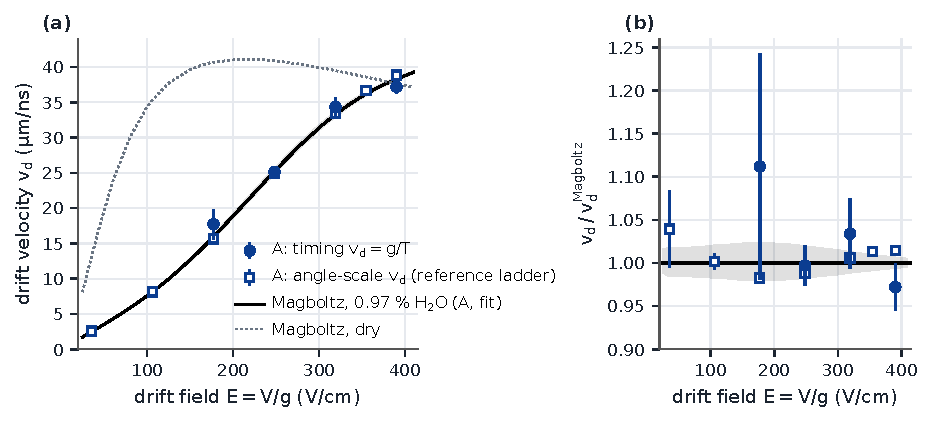
\includegraphics[width=0.66\linewidth]{gas_vE_all}
  \caption{Drift velocity against drift field, chamber~A. (a) Drift scan of 27 June: timing velocity $g/T$ from the
  duration of the drift column ($g=28.19$\,mm; filled circles) and angle-scale velocity from the reference tracks
  (no gap; open squares). Line: Magboltz for Ar/iC$_4$H$_{10}$ 95/5 with the water fitted to the timing
  velocity, 0.97\,\% [0.95, 0.99]; grey band, its 68\,\% interval; dotted, dry gas. (b) Ratio of the points to the
  curve.}
  \label{fig:vE}
\end{figure}

\subsection{The gas dries over hours}\label{sec:drying}
The water is not constant either. Through the night of 26--27 June the drift velocity of chambers C and D rose
steadily (\crefp{fig:drying}{a}), and inverted through the Magboltz curve at each chamber's field this is water
leaving the gas: from 1.47 to 0.76\,\% in chamber~C and from 0.68 to 0.35\,\% in chamber~D
(\crefp{fig:drying}{b}). The two chambers dry with one time shape (\crefp{fig:drying}{c}; correlation 0.975), but to
different plateaus, so they do not share one gas. Chamber~A dried in the same way, more slowly: its drift velocity rose by
1.8\,\% between Run~1 and the end of Run~2, from 35.8 to 36.6\,\textmu m/ns (\cref{app:gain}).

The consequence for a TPC of this kind is practical. With water at the per-cent level and changing by a factor of two
overnight, a drift velocity taken from the nominal gas or from an earlier run would put a scale error of tens of per
cent on every angle. The reconstruction therefore takes $\vd$ from each run's own data, and the velocity is, in
effect, the gas monitor of the bench.
\askStephan{Gas system on the bench: flow, materials, expected outgassing / water ingress? Were chambers C and D on one
gas line on 26 June?}

\begin{figure}[tbp]
  \centering
  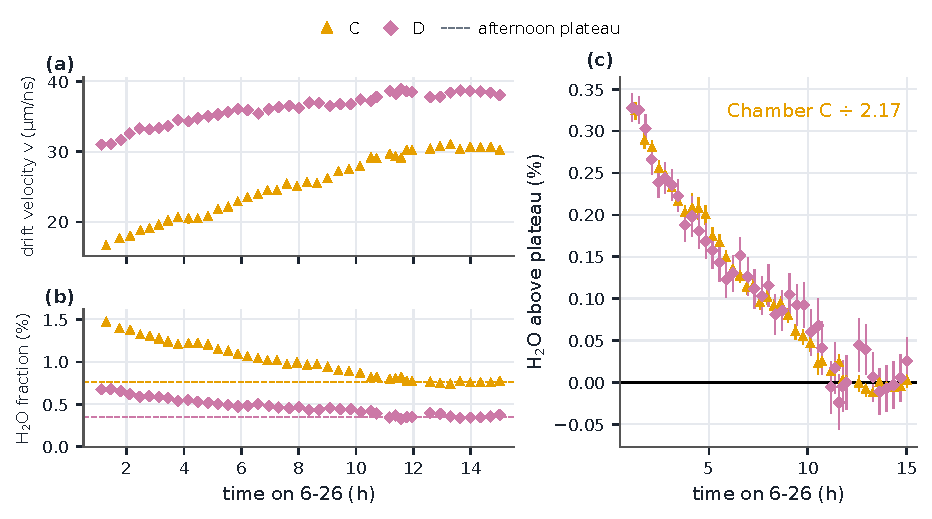
\includegraphics[width=0.88\linewidth]{gas_drying}
  \caption{The gas dries over the night of 26--27 June, chambers C and D. (a) Measured drift velocity (the angle-scale
  velocity, anchored to the timing velocity on the runs free of attachment), at 250 and 238\,V/cm respectively. (b)
  Water fraction inferred from (a) by inverting the Magboltz curve at each chamber's field; dashed, each chamber's
  plateau the following afternoon. (c) Excess over the plateau, chamber~C divided by 2.17: one time shape.}
  \label{fig:drying}
\end{figure}

\subsection{Oxygen: charge lost along the drift}\label{sec:attachment}
Water slows the drift; oxygen removes electrons from it. A track near normal incidence makes the same charge at every
depth, so its drift column, the summed signal against time, is a direct picture of the charge that survives from each
depth. On the bench the column of chamber~A is flat to its end (\crefp{fig:attach_charge}{a}): no charge is lost. In
the beam, chamber~E ran in two other mixtures, Ar/CF$_4$/iC$_4$H$_{10}$ and Ar/CO$_2$, and its column falls with drift
time in both. The same Magboltz model, now with drift, diffusion and attachment on a grid of water and oxygen, fits
these columns with 226 and 443\,ppm of oxygen; the same water with no oxygen stays flat and fails
(\crefp{fig:attach_charge}{b, c}). The method thus sees oxygen where there is some and none where there is none. The
water and oxygen of the beam test against time are in \cref{app:beam}.

\begin{figure}[tbp]
  \centering
  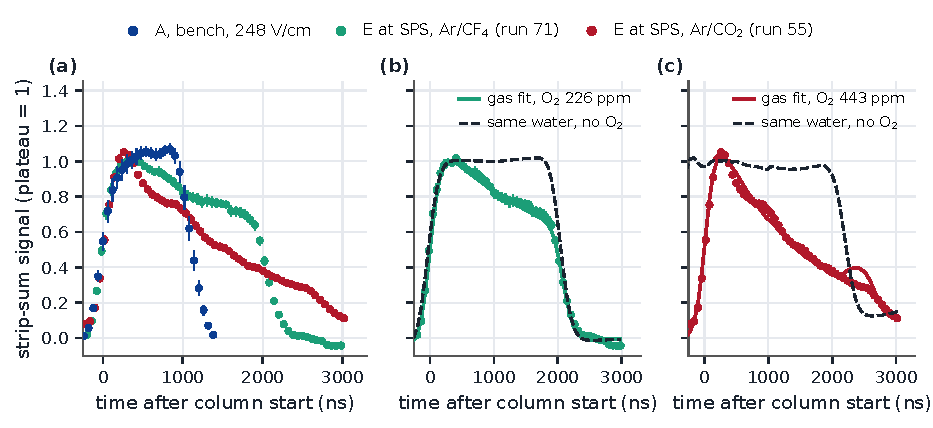
\includegraphics[width=\linewidth]{attachment_charge}
  \caption{Charge against drift time for tracks near normal incidence, each curve normalised to its plateau
  250--450\,ns after the start of the column. (a) Chamber~A on the bench (248\,V/cm) stays flat to the end of the
  column; chamber~E in the beam falls with drift time in both gases (Ar/CF$_4$/iC$_4$H$_{10}$ and Ar/CO$_2$, both at
  251\,V/cm): electrons from the far side of the gap are lost to attachment. (b, c) The two beam columns with the gas
  model (solid): Magboltz drift, diffusion and attachment, a fixed response of the electronics and a free time offset
  and amplitude, with water and oxygen fitted (226 and 443\,ppm of O$_2$). Dashed: the same water with no oxygen,
  which fails ($\chi^2$ 842 and 10\,600 against 49 and 258 for 55 points). The columns last longer in the beam because
  the drift is slower in these mixtures. The Ar/CO$_2$ data were zero-suppressed, and the model includes the distortion
  this causes.}
  \label{fig:attach_charge}
\end{figure}
